    \subsection{Wzór Eulera}
    \begin{theorem}
            Przez $v$ oznaczmy liczbę wierzchołków, $e$ liczbę krawędzi a $f$ liczbę ścian spójnego grafu planarnego $G$. Mamy:
            \begin{equation}
                v - e + f = 2
            \end{equation}
    \end{theorem}
    \begin{proof}
        Robimy sobie drzewo rozpinające naszego grafu $G$ (ważne założenie, że jest on spójny). Drzewa to dosyć przyjemna klasa grafów, bo jeśli mają $n$ wierzchołków to mają $n-1$ krawędzi. Ponadto mają tylko jedną ścianę (zewnętrzną). Zatem $f = 1$, a $e = v-1$. W takim razie dla drzewa rozpinającego naszego grafu planarnego zachodzi teza. Teraz zauważamy, że jak dodamy jakąś krawędź to to nadal zostaje równe 2, bo $f$ zwiększa się o jeden i $e$ zwiększa się o jeden. Dokładając zatem krawędź po krawędzi otrzymujemy wyjściowy graf planarny, w którym zachodzi teza. 
    \end{proof}

    \subsection{Liczba kolorująca}
    Pokażemy, że w dowolnym grafie planarnym $G$ istnieje wierzchołek o stopniu równym co najwyżej 5. Wtedy w oczywisty sposób ograniczymy liczbę kolorującą od góry przez 6 (bo w takim razie $\delta(G) \leq 5$ dla dowolnego grafu planarnego, więc będziemy mogli zastosować fajny wzór na liczbę kolorującą). Jeśli nie wiesz o jaki wzór mi chodzi, rekomenduję cofnięcie się do rozdziału o liczbie kolorującej, gdzie ten jest dowodzony. Do udowodnienia zostaje zatem pokazanie, że w każdym grafie planarnym istnieje wierzchołek o stopniu co najwyżej 5.

    \begin{theorem}
        W każdym grafie planarnym istnieje wierzchołek o stopniu co najwyżej 5.
    \end{theorem}
    \begin{proof}
        Załóżmy nie wprost, że tak nie jest. Ponadto zakładamy że graf jest spójny (bo jak nie jest, to prowadzimy rozumowanie dla grafu spójnego dla jakiegoś jego komponentu spójnego). Ze wzoru eulera mamy, że $v - e + f = 2$. Jednocześnie z założenia nie wprost mamy, że każdy wierzchołek ma stopień co najmniej 6. Stosujemy lemat o uściskach dłoni: 
        \begin{equation*}
            \sum_{u \in V} deg(u) = 2 \cdot |E|
        \end{equation*}
        Korzystając z założenia nie wprost, że dla dowolnego $u$ jest tak, że $(deg(u) \geq 6)$:
         \begin{equation*}
            \sum_{u \in V} deg(u) = 2 \cdot |E| \geq 6 \cdot v
        \end{equation*}
        czyli $e \geq 3v $. Teraz wykonuję fikołek, bo mówię że mój graf ma co najmniej 3 wierzchołki. Jeśli ma mniej, to w sumie teza jest oczywista. Jeśli ma co najmniej 3 wierzchołki zaś, to mogę wykonać bardzo ciekawą obserwację: mianowicie każda ściana ,,wydzielana'' jest przez co najmniej 3 krawędzie. W dodatku każda krawędź ma ,,kontakt'' z maksymalnie dwiema ścianami. 

        Teraz wykonuję bardzo śmieszną czynność, bowiem robię coś niezwykle poetyckiego, co wręcz prosi się o rysunek; na każdej ścianie ,,kładę'' 3 ,,monety''. Każda z tych monet idzie do różnych krawędzi. Jedna krawędź dostanie maksymalnie 2 monety, ale na każdej ścianie położono 3 monety. Stąd mam, że w grafie planarnym, który ma co najmniej 3 wierzchołki:
        \begin{equation*}
            2e \geq 3f
        \end{equation*}
        Jest to najbardziej machany dowód przez rysowanie który znam, ale jest on prezentowany również na wykładach. I okazuje się, że jak podstawimy tę własność do wzoru Eulera otrzymamy coś bardzo ciekawego. Mianowicie:
        \begin{equation*}
            v - e + f = 2
        \end{equation*}
        \begin{equation*}
            f = 2 - v + e
        \end{equation*}
        \begin{equation*}
           3f = 6 - 3v + 3e
        \end{equation*}
        \begin{equation*}
            6 - 3v + 3e = 3f \leq 2e
        \end{equation*}
         \begin{equation*}
            6 - 3v + 3e \leq 2e
        \end{equation*}
        \begin{equation*}
            6 - 3v + e \leq 0
        \end{equation*}
        \begin{equation*}
            e \leq 3v - 6
        \end{equation*}
        Zaraz chwilunia, ale z założenia nie wprost mieliśmy że $e \geq 3v$. Mielibyśmy wtedy, że $3v \leq 3v-6$ skąd $0 \leq -6$. Brzmi trochę jak sprzeczność. 
    \end{proof}
    
        \subsection{5-kolorowalność}
        \begin{theorem}[Ograniczenie górne na liczbę chromatyczną w grafach planarnych]
            W grafie planarnym $G$ zachodzi:
            \begin{equation}
                \chi(G) \leq 5
            \end{equation}
        \end{theorem}


            \begin{proof}
                Dowód przez indukcję. Zakładamy, że w każdym grafie planarnym jest tak, że istnieje wierzchołek o stopniu co najwyżej 5 (co zostało już udowodnione wcześniej). 

                Przypadek bazowy indukcji (graf planarny stanowiący po prostu jeden wierzchołek) jest trywialny. 

                Załóżmy teraz, że mam sobie graf planarny $G = (V,E)$. Biorę sobie wierzchołek $x$ taki, że ma stopień mniejszy lub równy 5. Z założenia indukcyjnego graf indukowany na wierzchołkach $V \setminus \{x\}$ można pokolorować 5 kolorami (lub mniej). Zakładam, że $x$ ma dokładnie 5 sąsiadów, bo jeśli ma ich mniej na pewno jest jakiś ,,wolny'' z 5 kolorów na które mogę go pokolorować i otrzymać poprawne kolorowanie. Sąsiadów $x$ oznaczam jako $v_1, v_2, v_3, v_4$ i $v_5$. Bez straty ogólności zakładamy, że w tej kolejności zgodnie z ruchem wskazówek zegara. Zakładam że sąsiad $v_i$ ma kolor $i$ (czyli że każdy sąsiad ma inny kolor; jeśli tak nie jest, to od razu mam poprawne kolorowanie, bo znowu biorę sobie ,,wolny'' kolor). 

                Zauważam teraz fajną rzecz: między dowolnymi dwoma sąsiadami $v_i$ i $v_j$ musi istnieć ścieżka z wierzchołkami o kolorach $i, j, i, \dots, i, j$. Wynika to z faktu, że gdyby takiej ścieżki nie było, to mógłbym wziąć sobie $v_i$ i przekolorować go na kolor $j$. Jego sąsiada w kolorze $j$ (o ile taki by istniał) na kolor $i$ i tak dalej. Otrzymałbym poprawne kolorowanie, ale $x$ miałby dwóch sąsiadów w kolorze $j$ (jeśli $v_i$ i $v_j$ są połączone to taki zabieg nadal daje poprawne kolorowanie, ale $v_j$ dostaje kolor $i$ i w sumie to nic nie osiągnąłem) i mógłbym mu dać kolor $i$. 

                Skoro tak, to między $v_1$ i $v_3$ istnieje taka ,,ścieżka dwukolorowa''. Zauważam jednak, że wtedy nie może istnieć taka ścieżka między $v_2$ i $v_4$ (znaczy zależy jak je rozrysujemy, ale jak zobaczycie rysunek to się wyjaśni o co mi chodzi -- pomysł jest taki, że $v_2$ jest poniekąd ,,odizolowany'' przez ścieżkę między $v_1$ a $v_3$). To oznacza, że zgodnie z opisaną powyżej procedurą mogę sobie po prostu przekolorować $v_2$ na kolor $4$, a wierzchołkowi $x$ dać kolor $2$, otrzymując poprawne kolorowanie. Nie mam pojęcia jak formaliści chcieliby to sformalizować, ale ci pewnie nadal siedzą nad definicją spaceru rozgałęziającego się w drzewie Steinera. 

                \begin{figure}[H]
                    \centering
                    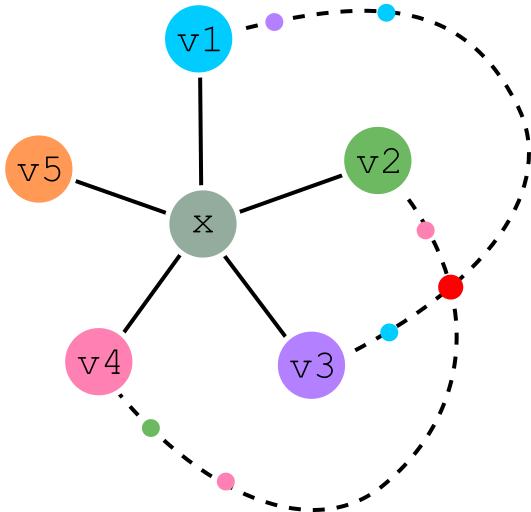
\includegraphics[scale=0.5]{images/graf_planarny.png}
                    \caption{Niemożliwe jest połączenie ,,ścieżką dwukolorową'' wierzchołka $v_2$ z $v_4$, jeśli takową już połączyliśmy wierzchołek $v_1$ z wierzchołkiem $v_3$.}
                \end{figure}
            
            \end{proof}

            \subsection{5-wybieralność}
            \epigraph{To było coś takiego?}{\textit{Student TCSu o 5-wybieralności, na chwilę przed wejściem na egzamin}}
            Jeśli myślisz że skoro tego nie ma w wymaganiach więc nie będzie na egzaminie, to się grubo mylisz. Byli już tacy, którzy na tym się przejechali. Nie wiem z czego wynika brak tego tematu w wymaganiach, ale czuję się zobowiązany go opisać. 

            \subsubsection{Co to jest w ogóle 5-wybieralność?}
            Podejrzewam, że spora część czytających zaczęła wyświetlać obrazek \textit{co.png} na twarzy gdy ujrzała frazę \textit{5-wybieralność}. Z tego względu pozwolę sobie zdefiniować, o co w ogóle tutaj chodzi. 

            Mówimy, że graf $G$ jest $k$-wybieralny, jeżeli po przydzieleniu każdemu wierzchołkowi jakiejś listy co najmniej $k$ różnych kolorów na które można go pokolorować, możliwe jest jego pokolorowanie (dla dowolnego takiego przydziału list). 
            
            \textit{Przykład.} Klika $K_3$ (znana wśród niektórych jako \textit{trójkąt}) jest 3-wybieralna. Klika dwudzielna $K_{3,3}$ nie jest natomiast $2$-wybieralna (mimo bycia $2$-kolorowalną). 

            \begin{figure}[H]
                \centering
                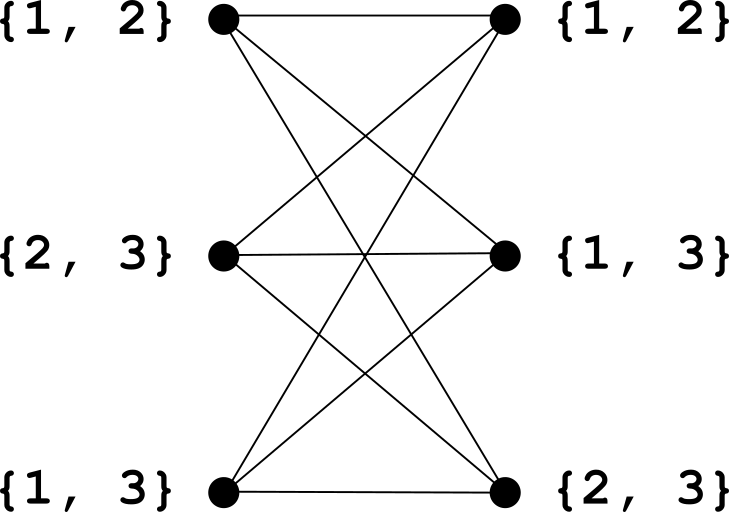
\includegraphics[scale=0.8]{images/K33.png}
                \caption{Klika dwudzielna $K_{3,3}$ z $2$-elementowymi listami takimi, że grafu nie da się pokolorować poprawnie.}
            \end{figure}

            Zauważmy również, że jeśli graf $G$ jest $k$-wybieralny, to $\chi(G) \leq k$; każdemu wierzchołkowi wystarczy dać listę $k$ kolorów od $1$ do $k$ (bo da się go pokolorować dla dowolnego przydziału list, w szczególności również i do takiego). 

            Najmniejsze takie $k$, że graf $G$ jest $k$-wybieralny, będziemy oznaczać jako $\chi_{_l}(G)$.

            \subsubsection{5-wybieralność grafów planarnych}
            Niech $G$ będzie grafem planarnym. Wtedy zachodzi:
            \begin{theorem}[O 5-wybieralności grafów planarnych]{
                \begin{equation} 
                    \chi_{_l}(G) \leq 5
                \end{equation}
            }               
            \end{theorem}

            \begin{proof}
                    Dowód przeprowadzimy indukcją, do której będziemy potrzebowali nieco silniejszych założeń niż tylko, że $G$ jest planarny i wszystkie listy są pięcioelementowe.
                    
                    Założenia, które czynimy:
                    \begin{enumerate}
                        \item Każda wewnętrzna ściana jest trójkątem.
                        \item Do ściany zewnętrznej przyległe są dwa sąsiadujące wierzchołki $u$ i $v$ takie, że
                        $$ |L(u)| = |L(v)| = 1, L(u) \neq L(v) $$
                        \item Pozostałe wierzchołki przyległe do ściany zewnętrznej mają listy długości 3
                        \item Wszystkie pozostałe wierzchołki grafu mają listy 5-elementowe
                    \end{enumerate}
                    
                    Zauważmy, że dowolny graf planarny wraz z listami 5-elementowymi jesteśmy w stanie przekształcić w graf spełniający powyższe warunki (dodając krawędzie i skracając odpowiednio listy), a uzyskane kolorowanie będzie poprawne w wyjściowym grafie.
                 
                    Robimy indukcję po liczbie wierzchołków; Widzimy, ze gdy $G$ ma co najwyżej 3 wierzchołki to teza w trywialny sposób zachodzi.

                    Rozpatrzmy teraz graf $G$ z jakimiś wierzchołkami $v, u$ które są na ścianie zewnętrznej. Rozważmy sąsiada $v$ ze ściany zewnętrznej (innego niż $u$). Nazwiemy go $w$. Rozpatrujemy teraz 2 przypadki: 

                    Gdy z $w$ wychodzi jakaś ,,cięciwa'', tj. krawędź łącząca się z innym wierzchołkiem na ścianie zewnętrznej różnym od dwóch, z którymi $w$ łączy się ,,normalnie''. Wtedy otrzymuję ,,podział'' grafu planarnego na 2 podgrafy. Z założenia indukcyjnego koloruję tę część, gdzie są wierzchołki $v$ i $u$. Zauważamy, że po takim pokolorowaniu drugi podgraf również spełnia nasze założenia, by go indukcyjnie pokolorować ($w$ i wierzchołek do którego prowadziła cięciwa mają już jakiś ustalony kolor; reszta wierzchołków na zewnątrz ma listy $3$-elementowe a wewnątrz $5$-elementowe; tu się nic nie zmieniło). Skoro tak, to go po prostu kolorujemy z założenia indukcyjnego i mamy poprawnie kolorowanie tą listą. Fajnie. 
                    
                    \begin{figure}[H]
                        \centering
                        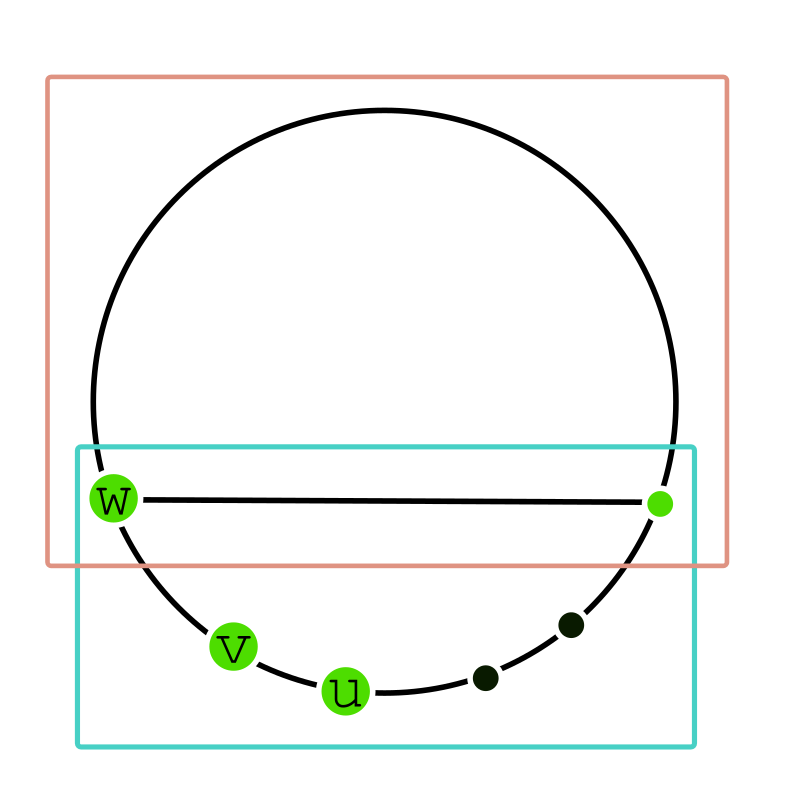
\includegraphics[scale=0.4]{images/5w1.png}
                        \caption{Z wierzchołka $w$ wychodzi ,,cięciwa'' która dzieli graf na 2 podgrafy; tę część, która zawiera $v$ i $u$ kolorujemy z założenia indukcyjnego. Wtedy $w$ i wierzchołek którego on ,,dotyka'' dostają już jakiś określony kolor, wobec czego dla drugiego podgrafu również możemy zastosować założenie indukcyjne.}
                    \end{figure}

                    W sytuacji, gdy z $w$ nie ma takiej ,,cięciwy'', sytuacja robi się nieco śmieszniejsza, ale w sumie to nie bardzo. Oznacza to tyle, że jeśli $w$ się łączy z jakimś wierzchołkiem, to ma on listę o 5 kolorach (chyba, że są to wierzchołki ,,na zewnątrz'', które będą maksymalnie 2). W takim razie wykonujemy bardzo sprytny plan: tworzymy dwuelementowy podzbiór listy $w$, taki że nie ma on jedynego koloru na który możemy pokolorować $v$ (zawsze możemy taki podzbiór utworzyć). Teraz każdemu sąsiadowi $w$ z listą pięcioelementową przyporządkowujemy listę trójelementową, taką że nie ma ona żadnego z tamtych dwóch kolorów. Jak się to narysuje to się okaże, że graf zawierający wszystkie wierzchołki poza $w$, z tak zdefiniowanymi listami, możemy pokolorować z założenia indukcyjnego (rysunek powinien rozjaśnić dlaczego). Teraz dokładamy z powrotem $w$; zauważamy, że musi mieć on co najmniej 1 taki kolor, że możemy go pokolorować (bo miał pulę 2 kolorów których nie współdzielił z nikim poza potencjalnie jednym wierzchołkiem, ale jak ten wierzchołek dostał kolor to na pewno zostanie nam 1 wolny). As you might've already guessed, nie mam bladego pojęcia jak to sformalizować. Whoopsie. Ale tak poza tym to właśnie dowiedliśmy co mieliśmy dowieść.

                    \begin{figure}[H]
                        \centering
                        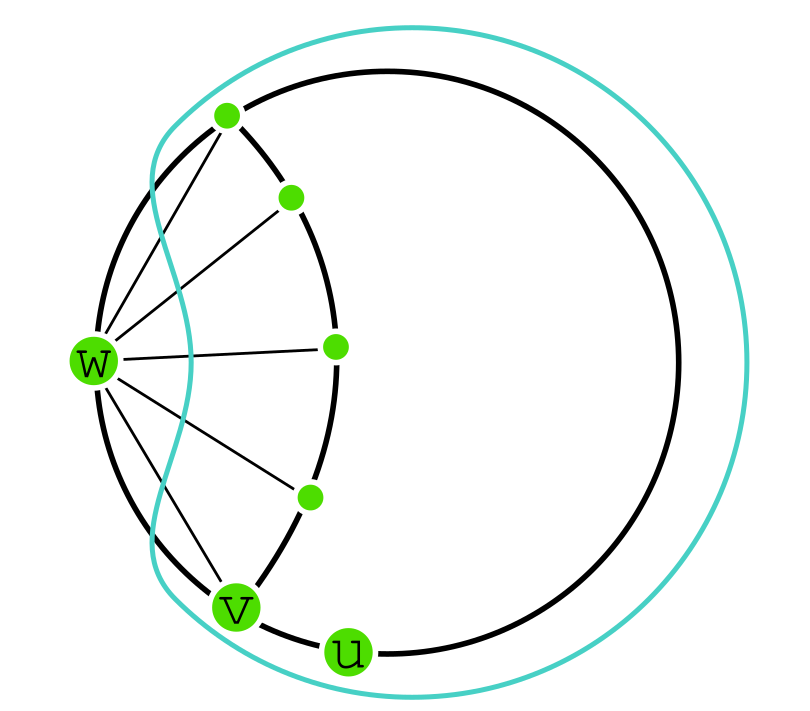
\includegraphics[scale=0.4]{images/5w2.png}
                        \caption{Z $w$ nie wycohdzi żadna ,,cięciwa'', więc wszystkie wierzchołki z którymi się łączy mają listę długości 5 (poza $v$ i jednym wierzchołkiem na okręgu). Modyfikujemy listy wierzchołkom których on dotyka i które mają 5 elementów, a potem go wywalamy; wtedy te z którymi się łączył będą na zewnątrz, i z założenia indukcyjnego możemy je pokolorować. }
                    \end{figure}
            \end{proof}